\subsection*{问题描述}

X 校最近打算美化一下校园环境。前段时间因为修地铁,X 校大门外种的行道树全部都被移走了。现在 X 校打算重新再种一些树,为校园增添一抹绿意。

X 校大门外的道路是东西走向的,我们可以将其看成一条数轴。在这条数轴上有 $n$ 个障碍物,例如电线杆之类的。虽然障碍物会影响树的生长,但是障碍物不一定能被随便移走,所以 X 校规定在障碍物的位置上{\heiti{不能}}种树。$n$ 个障碍物的坐标都是整数;如果规定向东为正方向,则 $n$ 个障碍物的坐标按照从西到东的顺序分别为 $a_1, a_2, \cdots, a_n$。X 校打算在 $\left[a_1, a_n\right]$ 之间种一些树,使得这些树看起来比较美观。

X 校希望,在一定范围内,树应该是等间隔的。更具体地说,如果把 $[a_1, a_n)$ 划分成一些区间 $\left[a_{p_1}, a_{p_2}\right),\cdots,\left[a_{p_{m-1}},a_{p_m}\right)$($1=p_1<p_2<\cdots<p_m=n$),那么每个区间 $\left[a_{p_i},a_{p_{i+1}}\right)$ 内需要至少种一棵树,且该区间内种的树的坐标连同区间端点 $a_{p_i}, a_{p_{i+1}}$ 应该构成一个等差数列。不同区间的公差,也就是树的间隔可以不相同。

例如,如果障碍物位于 $0, 2, 6$ 这三处,那么我们可以选择在 $[0, 2)$ 和 $[2, 6)$ 分别种树,也可以选择在 $[0, 6)$ 等间隔种树。如果是分别在 $[0, 2)$ 和 $[2, 6)$ 种树,由于每个区间内至少要种一棵树,坐标 $1$ 上必须种树;而 $[2, 6)$ 上的树可以按照 $1$ 的间隔种下,也可以按照 $2$ 的间隔种下。下图表示了这两种美观的种树方案,其中橙色的圆表示障碍物,绿色的圆表示需要在这个位置种树,箭头上的数字表示种下这棵树时对应的间隔为多少。

% <img alt="sample1_h.png" src="/RequireFile.do?fid=UXylvpoV"/>
\begin{figure}[H]
    \centering
    
\includegraphics[width=0.95\textwidth]{image/22/4-p-1.png}
    % \caption{神经元 $v$ 变量随时间变化的曲线}
\end{figure}

对区间 $[0, 2)$ 和 $[2, 6)$ 分别以 $1$ 和 $2$ 的间隔种树是美观的

% <img alt="sample2_h.png" src="/RequireFile.do?fid=G97DdvfC"/>
\begin{figure}[H]
    \centering
    
\includegraphics[width=0.95\textwidth]{image/22/4-p-2.png}
    % \caption{神经元 $v$ 变量随时间变化的曲线}
\end{figure}

对区间 $[0, 2)$ 和 $[2, 6)$ 分别以 $1$ 的间隔种树也是美观的

而如果选择在 $[0, 6)$ 区间等间隔种树,我们只能以 $3$ 的间隔种树,因为无论是选择间隔 $1$ 或者间隔 $2$,都需要在坐标 $2$ 上种树,而这个位置已经有障碍物了。下图分别表示了间隔为 $3, 2, 1$ 时的种树情况,红色箭头表示不能在这里种树。

% <img alt="sample3_h.png" src="/RequireFile.do?fid=dAQwSTuu"/>
\begin{figure}[H]
    \centering
    
\includegraphics[width=0.95\textwidth]{image/22/4-p-3.png}
    % \caption{神经元 $v$ 变量随时间变化的曲线}
\end{figure}

对区间 $[0, 6)$ 以 $3$ 的间隔种树是美观的

% <img alt="sample4_h.png" src="/RequireFile.do?fid=hpTkShxA"/>
\begin{figure}[H]
    \centering
    
\includegraphics[width=0.95\textwidth]{image/22/4-p-4.png}
    % \caption{神经元 $v$ 变量随时间变化的曲线}
\end{figure}

对区间 $[0, 6)$ 以 $2$ 的间隔种树是不美观的

% <img alt="sample5_h.png" src="/RequireFile.do?fid=oNrrpgBz"/>
\begin{figure}[H]
    \centering
    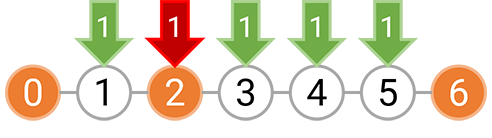
\includegraphics[width=0.95\textwidth]{image/22/4-p-5.png}
    % \caption{神经元 $v$ 变量随时间变化的曲线}
\end{figure}

对区间 $[0, 6)$ 以 $1$ 的间隔种树也是不美观的

一般地,给定一个区间 $[a_l, a_r)$,对于树的坐标的集合 $T\subset(a_l, a_r)$($T\subset\mathbb{Z}$),归纳定义 $T$ 在 $[a_l, a_r)$ 上是{\heiti{美观的}}:

\begin{enumerate}

\item 如果 $T\ne \emptyset$,$T\cap \left\{a_l, a_{l+1}, \cdots, a_r\right\}=\emptyset$,并且存在一个公差 $d\ge 1$,使得 $T\cup\left\{a_l, a_r\right\}$ 中的元素按照从小到大的顺序排序后,可以构成一个公差为 $d$ 的等差数列(显然,这个等差数列的首项为 $a_l$,末项为 $a_r$),则 $T$ 在 $\left[a_l, a_r\right)$ 上是美观的;

\item 如果 $T\cap \left\{a_l, a_{l+1}, \cdots, a_r\right\}=\emptyset$,并且存在一个下标 $m$($l<m<r$),使得 $T\cap\left(a_l, a_m\right)$ 在 $\left[a_l, a_m\right)$ 上是美观的,且 $T\cap\left(a_m, a_r\right)$ 在 $\left[a_m, a_r\right)$ 上是美观的,则 $T$ 在 $\left[a_l, a_r\right)$ 上是美观的。

\end{enumerate}

根据这一定义,空集在任意区间上都不是美观的;另外,如果存在下标 $i$ 使得 $a_i \in T$,那么 $T$ 一定不是美观的。

我们称两种种树的方案是{\heiti{本质不同的}},当且仅当两种方案中,种树的坐标集合不同。请帮助 X 校对 $\left[a_1, a_n\right)$ 求出所有本质不同的美观的种树方案。当然,由于方案可能很多,你只需要输出总方案数对 $10^9+7$ 取模的结果。


\subsection*{输入格式}

输入的第一行包含一个正整数 $n$,表示障碍物的数量。

输入的第二行包括 $n$ 个非负整数 $a_1, \cdots, a_n$,表示每个障碍物的坐标。

保证对 $i=1, 2, \cdots, n-1$,$a_i < a_{i+1}$。


\subsection*{输出格式}

输出一个非负整数,表示本质不同的美观的种树方案的数量对 $10^9+7$ 取模的结果。


